\documentclass{article}

\usepackage{arxiv}
\usepackage{graphicx}
\usepackage{amsmath}
\usepackage{booktabs}
\usepackage{tabularx}
\usepackage{array}
\usepackage{longtable}
\usepackage{hyperref}
\usepackage{url}

\title{Bitres System Design Document: Functional Architecture and Weak Governance}
\author{Invariant Core\\
\texttt{invariantcore@gmail.com}\\
\url{https://www.bitres.org}}
\date{\today}

\renewcommand{\shorttitle}{Bitres System Design Document: Functional Architecture and Weak Governance}
\hypersetup{
  colorlinks=true,
  linkcolor=blue,
  citecolor=blue,
  urlcolor=blue,
  pdftitle={Bitres System Design Document: Functional Architecture and Weak Governance},
  pdfauthor={Bitres Labs}
}

\setlength{\parindent}{2em}
\setlength{\parskip}{0pt}

% Remove Preprint text
\renewcommand{\headeright}{}
\renewcommand{\undertitle}{}

\begin{document}
\maketitle

\section{Document Objectives}
This document is written based on the Bitres whitepaper: ``Bitres: A Decentralized Stablecoin System Collateralized by Bitcoin''. The document elaborates on the overall architecture and design objectives of Bitres, as well as the economics of three tokens, including the stablecoin BTD, bond token BTB, and governance token BRS. The document focuses on token supply, price pegging, collateral safety thresholds, and incentive parameters, aiming to provide a requirements specification consistent with the whitepaper for subsequent economic analysis and implementation iterations, without relying on any specific implementation's function or variable names.

\subsection{Design Philosophy: Functional and Weak Governance}
The system adopts a design philosophy of \textbf{functional programming} and \textbf{weak governance}, aiming to achieve immutability and predictability similar to Bitcoin:
\begin{itemize}
  \item \textbf{Functional Architecture}: Core business logic is abstracted into pure function libraries, with minimal contract state. Price calculation, deviation validation, IUSD adjustment, and other algorithms are solidified as mathematical formulas, independent of mutable state, ensuring behavioral determinism.
  \item \textbf{Weak Governance Principle}: The system hard-codes the vast majority of parameters as immutable constants at launch, retaining only minimal governance capability for a very small number of necessary parameters. Governable parameters must satisfy four strict security mechanisms: boundary checks, cooldown periods, whitelist restrictions, and event logging.
  \item \textbf{Parameter Classification System}:
    \begin{itemize}
      \item \textit{Static Constants} (constant): Mathematical constants, precision, time parameters, etc., determined at compile time
      \item \textit{Immutables} (immutable): Core addresses, oracle IDs, inflation parameters, etc., set at deployment and never changeable
      \item \textit{Governable Parameters} (governable): A very small number of parameters requiring flexible adjustment, subject to strict constraints
    \end{itemize}
\end{itemize}
This design ensures the system behaves as close to Bitcoin's immutability as possible while retaining minimal flexibility to handle extreme situations.

\section{Overall Structure Overview}
The system contains a custody module, a minting and redemption module, a parameter configuration module, plus two incentive modules for interest rates and mining.
\begin{itemize}
  \item \textbf{Collateral Custody Module}: Stores all WBTC collateral and manages the BTD and BRS inventory accumulated within the system;
  \item \textbf{Minting and Redemption Module}: Responsible for BTC\,$\leftrightarrow$\,BTD exchange, also issues new bond token BTB when collateral is insufficient, and can use governance token BRS stored in the custody module for compensation;
  \item \textbf{Configuration and Oracle Module}: Maintains asset addresses, decentralized price pools, off-chain price sources, interest rates, and price threshold parameters;
  \item \textbf{Interest Rate Control Module}: Updates the annualized yield rates for BTD and BTB staking based on market prices and collateral ratio;
  \item \textbf{Mining Module}: Releases governance tokens according to a four-year halving system and distributes rewards to the ecosystem fund, team, and liquidity providers.
\end{itemize}

\section{Price Pegging and Collateral Ratio}
\subsection{Target Unit of Account}
The stablecoin BTD maintains a peg to ``Ideal USD'' (IUSD):
\begin{equation}
1\,\text{BTD} = 1\,\text{IUSD}=\frac{\text{PCE}_n}{\text{PCE}_0\times1.02^{n/12}}\,\text{USD}.
\end{equation}
IUSD is initially priced at 1 USD, with a target annual inflation rate of 2\%, i.e., monthly inflation rate $\approx 0.165\%$. The initial month's Personal Consumption Expenditure price index is $\text{PCE}_0$, and the current month's Personal Consumption Expenditure price index is $\text{PCE}_n$, where n represents the nth month after the initial month. When PCE data is higher than the target inflation, IUSD will depreciate accordingly, and vice versa, thereby achieving a long-term monetary policy of 2\% annual inflation.

\subsubsection{Inflation Parameter Solidification}
\textbf{The 2\% annual inflation rate of IUSD is the system's core monetary policy commitment, fully solidified at deployment}:
\begin{itemize}
  \item \textbf{Immutable Constants}: The annual inflation rate (2\% = 0.02) and monthly growth factor ($1.02^{1/12} \approx 1.001651581301920174$) are set as immutable parameters in the constructor, never modifiable after deployment.
  \item \textbf{PCE Oracle Solidification}: The data source address and precision configuration for the US PCE (Personal Consumption Expenditure) price index are solidified at deployment, preventing data source tampering.
  \item \textbf{Functional Adjustment Factor Calculation}: The calculation logic for the IUSD adjustment factor is encapsulated as a pure function library, deterministically calculated based on on-chain PCE data and solidified inflation targets through mathematical formulas, independent of mutable state.
  \item \textbf{Emergency Override Mechanism}: Only in extreme situations such as PCE oracle failure, authorized addresses are allowed to manually override the IUSD value, but subject to strict restrictions: deviation not exceeding 5\%, interval of at least 7 days, and complete event log recording.
\end{itemize}
This design ensures that IUSD's monetary policy is as predictable and immutable as Bitcoin's fixed supply.

\subsection{Price Sources and Validation}
BTC price references both:
\begin{enumerate}
  \item Off-chain oracle (using Chainlink BTC/USD feed as benchmark);
  \item Decentralized exchange pool (WBTC/USDC trading pair).
\end{enumerate}
If the deviation between the two exceeds 1\%, the minting process will terminate directly. The prices of bond and governance tokens are also converted to USD through their respective DEX trading pairs for calculating compensation, interest rates, and buyback amounts.

\subsubsection{Oracle Parameter Governance Strategy}
Oracle configuration follows a balanced approach between security and flexibility:
\begin{itemize}
  \item \textbf{Governable External Addresses}: External oracle addresses (Chainlink feeds, Pyth, Redstone) and DEX pool addresses are governable to allow upgrades when external systems change. Changes are subject to timelock delay (7 days) and whitelist restrictions.
  \item \textbf{Immutable Core Logic}: Price ID formats, precision configuration, and calculation algorithms are immutable after deployment.
  \item \textbf{Deviation Threshold Governance}: Price deviation tolerance is governable, but can only be \textit{unidirectionally tightened} (from 1\% to stricter values), and is constrained by cooldown period (1 day) and range limits (0.5\%--5\%).
  \item \textbf{Functional Price Aggregation}: Price calculation logic is encapsulated as a pure function library, including multi-source median calculation, deviation validation, etc., independent of mutable state, ensuring the algorithm is transparent and immutable.
\end{itemize}

\subsection{Collateral Ratio Definition}
The system measures security boundaries using Collateral Ratio (CR):
\begin{equation}
\text{CR} = \frac{\text{BTC Holdings} \times P_{\text{BTC}}}{\text{BTD Equivalent Total Amount} \times P_{\text{IUSD}}}.
\end{equation}
Where \textbf{BTD Equivalent Total Amount} is defined as:
\begin{equation}
\text{BTD Equivalent Total Amount} = \text{BTD Supply} + \text{All stBTD converted to BTD Amount}.
\end{equation}
$P_{\text{BTC}}$ represents the price of BTC, and $P_{\text{IUSD}}$ represents the price of IUSD. When CR $\geq 100\%$, the system is fully backed by BTC; when CR $< 100\%$, the gap is absorbed through newly issued BTB and treasury BRS.

\section{BTD: Stablecoin}
\subsection{Token Overview}
\begin{tabularx}{\textwidth}{l X}
\toprule
Name & Bitcoin Dollar \\
Symbol & BTD \\
Token Standard & ERC20, extended to support upgradability, burnable, pausable, Permit, custody and blacklist control \\
Total Supply & Unlimited, dynamically adjusted based on collateral demand and interest distribution \\
Precision & 18 decimals \\
Production Mechanism & Issued by the minting and redemption module when WBTC is collateralized, and minted when the staking interest module distributes interest \\
Issuer & Bitres \\
Collateral & WBTC \\
Use Case & Stable settlement asset pegged to IUSD, used for payments, liquidation, and intra-system collateral \\
\bottomrule
\end{tabularx}

\subsection{Supply and Fees}
After a user deposits 1 WBTC, $Q_{\text{BTD}}$ stablecoins are minted according to the validated price:
\begin{align}
Q_{\text{BTD}} &= \frac{ P_{\text{BTC}}}{P_{\text{IUSD}}}. \\
\text{Fee} &= Q_{\text{BTD}} \times 0.5\%.
\end{align}
The fee is additionally minted and not collected from the user, and will be fully transferred to treasury inventory. BTD has no total supply cap; its supply is entirely driven by collateral and interest rate policy.

\subsection{Redemption and Gap Handling}
When a user deposits 1 BTD into the system for redemption, the user's BTD will first be burned, then assets are returned based on the current collateral ratio:
\begin{itemize}
  \item \textbf{CR $\geq 100\%$}: All converted to $Q_{\text{BTC}}$ WBTC and returned:
\begin{align}
Q_{\text{BTC}} &= \frac{ P_{\text{IUSD}}}{P_{\text{BTC}}}. \\
\end{align}
  \item \textbf{CR $< 100\%$}:
    \begin{enumerate}
      \item First return $x$ WBTC,
      \begin{equation}
      x = \frac{\text{BTC Holdings}}{\text{BTD Equivalent Total Amount}}.
      \end{equation}
      \item Then newly issue $y$ BTB,
      \begin{equation}
      y = \frac{(1-\text{CR}) \times P_{\text{IUSD}}}{max(P_{\text{BTB}},P_{\text{BTB,min}})}.
      \end{equation}
Where $P_{\text{BTB}}$ is the market price of BTB, and $P_{\text{BTB,min}}$ is the system-specified minimum price of BTB.
      \item If the market price $P_{\text{BTB}}$ is below the bond floor price $P_{\text{BTB,min}}$, the difference is compensated with $z$ BRS,
      \begin{equation}
      z = \frac{(1-\text{CR}) \times P_{\text{IUSD}}\times (P_{\text{BTB,min}}-P_{\text{BTB}})}{P_{\text{BTB,min}}\times P_{\text{BRS}}}.
      \end{equation}
    \end{enumerate}
\end{itemize}
The BRS used for compensation comes from treasury inventory and is not newly minted. Thus, each 1 BTD redemption request is split into ``immediately returned BTC + newly minted BTB + final backstop BRS''.
In the initial setup, the system defaults to $P_{\text{BTB,min}} = 0.5\,\text{BTD}$.

\subsection{Staking Interest}
BTD can earn deposit interest in the staking pool. The deposit rate is determined algorithmically based on BTD's market price relative to IUSD, using a Sigmoid function to achieve smooth transitions. When BTD price falls below the anchor (1 IUSD), higher rates attract deposits; when price rises above the anchor, lower rates discourage excessive supply. See Section~\ref{sec:interest-rates} for detailed formulas and parameters.

Interest accumulates per second and is paid to stakers through BTD minting. The operator can levy an additional fee rate on interest income (default 10\%, adjustable by governance).

\section{BTB: Bond Token}
\subsection{Token Overview}
\begin{tabularx}{\textwidth}{l X}
\toprule
Name & Bitcoin Bond \\
Symbol & BTB \\
Token Standard & ERC20, extended to support upgradability, burnable, pausable, custody and blacklist control \\
Total Supply & Unlimited, dynamically changes based on collateral gap and interest rate incentives \\
Precision & 18 decimals \\
Production Mechanism & Automatically minted during redemption processes when collateral ratio is insufficient, and minted when the staking interest module distributes interest \\
Issuer & Bitres \\
Collateral & BTD \\
Use Case & Deferred payment debt certificate, stabilizes collateral ratio and recovers system risk premium \\
\bottomrule
\end{tabularx}

\subsection{Issuance and Pricing}
BTB represents the system's deferred payment promise to stablecoin holders:
\begin{itemize}
  \item When the collateral ratio is below 100\%, bonds are minted at the real-time IUSD/BTB price during the redemption process;
  \item If the market price falls below 0.5 BTD, the system still issues BTB at the 0.5 BTD face value and compensates the discount with BRS, preventing losses from being further amplified due to insufficient market depth;
  \item Outside of redemption scenarios, BTB can only be minted for staking interest in the staking pool.
\end{itemize}

\subsection{Redemption Conditions}
When the collateral ratio recovers to above 100\%, bond holders can exchange stablecoins at a rate of $1 \;\text{BTB} =1 \;\text{BTD}$:
\begin{equation}
\text{Redeemable BTD Upper Limit} = (\text{CR}-1) \times \text{BTD Equivalent Total Amount}.
\end{equation}
Redemption burns the corresponding BTB until the system returns to exactly 100\% collateralization.

\subsection{Staking Interest Rate Policy}
The bond rate is determined algorithmically based on two factors: (1) the system's collateral ratio (CR), which affects the base rate, and (2) BTB's market price relative to BTD, which determines rate adjustments. When $CR \geq 100\%$, BTB can be redeemed 1:1 for BTD, so risk is low. When $CR < 100\%$, BTB cannot be redeemed, so holders bear higher risk and deserve higher compensation through an increased base rate.

Similar to BTD, the rate uses a Sigmoid function for smooth price-based adjustment. When BTB price falls below the anchor (1 BTD), higher rates attract bond holders; when price rises above the anchor, lower rates apply. Interest is distributed by minting BTB. The maximum rate is capped at 20\% to prevent excessive token inflation. See Section~\ref{sec:interest-rates} for detailed formulas and parameters.

\section{BRS: Governance Token}
\subsection{Token Overview}
\begin{tabularx}{\textwidth}{l X}
\toprule
Name & Bitcoin Reserve System Token \\
Symbol & BRS \\
Token Standard & ERC20, extended to support upgradability, burnable, pausable, Permit, custody, blacklist and vote accounting \\
Total Supply & Capped at 2.1 billion, four-year halving mining mechanism \\
Precision & 18 decimals \\
Production Mechanism & Issued by mining module with four-year halving \\
Issuer & Bitres \\
Collateral & Treasury net assets after deducting total BTD and BTB liabilities \\
Use Case & Governance voting, risk buffer and ecosystem incentives, supporting treasury buybacks and system upgrades \\
\bottomrule
\end{tabularx}

\subsection{Mining Mechanism}
BRS is used for governance voting, compensation in extreme situations, and ecosystem incentives. Core production parameters are as follows:
\begin{itemize}
  \item \textbf{Total Supply Cap:} $2.1\times 10^9$ tokens;
  \item \textbf{Halving Cycle:} Every 4 years;
  \item \textbf{First Cycle Release:} $1.05\times 10^9$ tokens, corresponding to initial production of approximately $8.33$ tokens/second;
  \item \textbf{Fund Allocation:} By default, three addresses receive Treasury 20\%, Foundation 10\%, Team 10\% of new production (totaling 40\%, adjustable by governance), with the remaining 60\% used to reward stakers.
\end{itemize}
When cumulative issuance reaches the cap, mining rewards terminate.

\subsubsection{Initial Mining Pool Configuration}
The 60\% portion of BRS mining rewards distributed to stakers is implemented through multiple mining pools to incentivize different types of liquidity provision and token staking behavior. Initial mining pool configuration is as follows:

\textbf{1. LP Liquidity Mining Pools (45\%):}
\begin{itemize}
  \item \textbf{BRS/BTD LP Pool:} 15\% allocation weight, incentivizes BRS and BTD liquidity pairing
  \item \textbf{BTD/USDC LP Pool:} 15\% allocation weight, provides mainstream on-ramp for stablecoin
  \item \textbf{BTB/BTD LP Pool:} 15\% allocation weight, promotes bond token and stablecoin swap liquidity
\end{itemize}

\textbf{2. Single Token Staking Mining Pools (15\%):}
\begin{itemize}
  \item \textbf{USDC Pool:} 1\% allocation weight, provides additional yield for USDC holders
  \item \textbf{USDT Pool:} 1\% allocation weight, supports another mainstream stablecoin
  \item \textbf{WBTC Pool:} 1\% allocation weight, encourages Bitcoin asset participation
  \item \textbf{ETH Pool:} 1\% allocation weight, supports Ethereum asset participation
  \item \textbf{stBTD Pool:} 3\% allocation weight, users deposit BTD into ERC4626 vault to receive stBTD share tokens, staking stBTD yields dual returns (BTD interest through automatic share price growth + BRS mining rewards)
  \item \textbf{stBTB Pool:} 3\% allocation weight, users deposit BTB into ERC4626 vault to receive stBTB share tokens, staking stBTB yields dual returns (BTB interest through automatic share price growth + BRS mining rewards)
  \item \textbf{BRS Pool:} 5\% allocation weight, encourages long-term holding of governance tokens
\end{itemize}

\textbf{stToken Dual Yield Mechanism Explanation:}

BTD and BTB implement dual yield mechanisms using the ERC4626 tokenized vault standard. Users participate through the following process:

\begin{enumerate}
  \item \textbf{Deposit Phase:} Users deposit BTD/BTB into the corresponding vault contract and receive stBTD/stBTB share tokens at the current exchange rate;
  \item \textbf{Interest Accumulation:} The stToken share price automatically grows over time, reflecting accumulated interest earnings. Interest earnings come from:
    \begin{itemize}
      \item stBTD: Deposit interest following the federal funds rate
      \item stBTB: Bond interest dynamically adjusted based on market price
    \end{itemize}
  \item \textbf{Further Staking:} Users can stake stBTD/stBTB into the BRS mining pool (FarmingPool) to earn additional BRS mining rewards;
  \item \textbf{Dual Yield:} Ultimately achieving ``one deposit, dual yields'':
    \begin{itemize}
      \item BTD → stBTD → BTD interest (auto-compounding) + BRS mining rewards
      \item BTB → stBTB → BTB interest (auto-compounding) + BRS mining rewards
    \end{itemize}
\end{enumerate}

The advantage of stToken design: Funds only need to be transferred once, interest auto-compounds through share price appreciation, and users can redeem principal plus interest at any time without manual claiming.

\textbf{Initial Mining Pool Allocation Weight Table:}
\begin{center}
\begin{tabular}{clcc}
\toprule
Pool ID & Type and Token & Allocation Weight & Percentage \\
\midrule
0 & BRS/BTD LP & 15 & 15\% \\
1 & BTD/USDC LP & 15 & 15\% \\
2 & BTB/BTD LP & 15 & 15\% \\
3 & USDC Single Token & 1 & 1\% \\
4 & USDT Single Token & 1 & 1\% \\
5 & WBTC Single Token & 1 & 1\% \\
6 & ETH Single Token & 1 & 1\% \\
7 & stBTD Single Token Staking & 3 & 3\% \\
8 & stBTB Single Token Staking & 3 & 3\% \\
9 & BRS Single Token & 5 & 5\% \\
\midrule
\multicolumn{2}{l}{\textbf{Total (Stakers)}} & \textbf{60} & \textbf{60\%} \\
\multicolumn{2}{l}{\textbf{Treasury}} & -- & \textbf{20\%} \\
\multicolumn{2}{l}{\textbf{Foundation}} & -- & \textbf{10\%} \\
\multicolumn{2}{l}{\textbf{Team}} & -- & \textbf{10\%} \\
\midrule
\multicolumn{2}{l}{\textbf{Total}} & -- & \textbf{100\%} \\
\bottomrule
\end{tabular}
\end{center}

This configuration can be dynamically adjusted through the governance module to adapt to market changes and ecosystem development needs.

\subsection{Price Support and Buyback}
The treasury can use accumulated BTD to buy back BRS in the secondary market, with purchased BRS retained in the treasury to form BRS inventory. This process does not rely on token burn functions but adjusts circulating supply through treasury management. Treasury BRS inventory mainly comes from:
\begin{itemize}
  \item \textbf{Mining Allocation:} 20\% of mining output is automatically allocated to the treasury address;
  \item \textbf{Fee Buyback:} Using BTD fees collected by the system to buy back BRS in the market.
\end{itemize}
Treasury BRS inventory is used both for price support and as the funding source for BRS compensation functionality.

\subsection{Compensation Function}
When collateral is insufficient and bond prices are below face value, redeemers receive additional BRS compensation. The compensation amount depends on the degree of bond price deviation and the BRS/BTD exchange rate, serving as the last line of defense in the BTD price pegging mechanism's three-layer defense system.

\textbf{Important Mechanism Explanation:}
\begin{itemize}
  \item \textbf{Compensation Source:} BRS compensation is not from newly minted tokens, but transferred from treasury BRS inventory, ensuring the 2.1 billion total supply cap is not breached;
  \item \textbf{Natural Limitation:} Compensation is constrained by available treasury balance. When treasury BRS inventory is insufficient, compensation amount automatically reduces to inventory balance; when inventory is depleted, compensation stops;
  \item \textbf{Risk Buffer:} The treasury's BRS inventory represents the system's extreme risk tolerance capacity. During normal periods, the treasury accumulates BRS; during crisis periods, BRS is released for compensation, forming a natural risk buffer mechanism.
\end{itemize}

\section{Interest}
\subsection{stToken Vault Mechanism}
The system uses the ERC4626 tokenized vault standard to implement interest accumulation and distribution. User participation process is as follows:

\subsubsection{Deposit and Share Minting}
\begin{itemize}
  \item Users deposit BTD or BTB into the corresponding vault contract (stBTD Vault or stBTB Vault);
  \item The vault calculates and mints the corresponding amount of share tokens (stBTD or stBTB) at the current exchange rate and returns them to the user;
  \item Initial exchange rate is 1:1, i.e., first deposit of 1 BTD yields 1 stBTD share.
\end{itemize}

\subsubsection{Interest Accumulation Mechanism}
Interest is not implemented by minting additional tokens to user accounts, but automatically accumulated through share price appreciation:
\begin{itemize}
  \item \textbf{stBTD Vault:} Interest Pool accumulates BTD interest per block, interest enters vault total assets;
  \item \textbf{stBTB Vault:} Interest Pool accumulates BTB interest per block, interest enters vault total assets;
  \item \textbf{Share Price Appreciation:} Total assets increase but total shares remain unchanged, causing each share to correspond to more assets, achieving auto-compounding;
  \item \textbf{Claim Method:} When users redeem stToken, they receive principal plus interest in BTD/BTB at the current exchange rate.
\end{itemize}

Example: User deposits 100 BTD and receives 100 stBTD. After one year (assuming 5\% annual rate), redemption yields 105 BTD, while stBTD quantity remains 100.

\subsubsection{Interest Rates}
\label{sec:interest-rates}
Both BTD and BTB interest rates are determined algorithmically using Sigmoid functions based on market prices and an internal base rate that varies with collateral ratio (CR).

\paragraph{Base Rate Formula}
Both BTD and BTB use a CR-based base rate formula:
\begin{equation}
r_{base}(CR) = r_{default} \times (1 + \Delta_{CR})
\end{equation}

Where $r_{default} = 5\%$ is the governance-adjustable default rate (anchor point when CR = 100\%).

The $\Delta_{CR}$ adjustment factor varies by CR:
\begin{equation}
\Delta_{CR} = \begin{cases}
-0.6 \times \dfrac{CR - 1}{0.5} & CR > 1 \quad \text{(rate decreases)} \\[0.5em]
0 & CR = 1 \quad \text{(anchor point)} \\[0.5em]
\dfrac{1 - CR}{0.8} \times k & 0.2 \leq CR < 1 \quad \text{(rate increases)}
\end{cases}
\end{equation}

Where $k = 1$ for BTD and $k = 3$ for BTB (higher risk compensation).

\paragraph{BTD Deposit Rate}
BTD uses a Sigmoid function with the following parameters:
\begin{itemize}
  \item $r_{max} = 10\%$: Maximum deposit rate
  \item $r_{min} = 2\%$: Minimum deposit rate (reached at CR $\geq 150\%$)
  \item $\alpha = 25$: Sigmoid steepness parameter (price range 0.8--1.2)
  \item Range: 2\%--10\%
\end{itemize}

\begin{center}
\begin{tabular}{ccc}
\toprule
Collateral Ratio & $\Delta_{CR}$ & Base Rate \\
\midrule
$\geq 150\%$ & $-0.6$ & $2\%$ (minimum) \\
$100\%$ & $0$ & $5\%$ (default) \\
$60\%$ & $0.5$ & $7.5\%$ \\
$20\%$ & $1.0$ & $10\%$ (maximum) \\
\bottomrule
\end{tabular}
\end{center}

The final BTD rate is calculated using:
\begin{equation}
r_{BTD}(P, CR) = r_{max} \cdot S\left(-\alpha \cdot (P - 1) + \beta(CR)\right)
\end{equation}

Where $\beta(CR) = \ln\left(\frac{r_{base}(CR)}{r_{max} - r_{base}(CR)}\right)$ and $S(x) = \frac{1}{1 + e^{-x}}$ is the Sigmoid function.

\paragraph{BTB Bond Rate}
BTB uses a 3x $\Delta_{CR}$ multiplier for higher risk compensation:
\begin{itemize}
  \item $r_{max} = 20\%$: Maximum bond rate
  \item $r_{min} = 2\%$: Minimum bond rate (reached at CR $\geq 150\%$)
  \item $\alpha = 10$: Sigmoid steepness parameter (price range 0.5--1.5)
  \item Range: 2\%--20\%
\end{itemize}

\begin{center}
\begin{tabular}{ccc}
\toprule
Collateral Ratio & $\Delta_{CR}$ (with 3x) & Base Rate \\
\midrule
$\geq 150\%$ & $-0.6$ & $2\%$ (minimum) \\
$100\%$ & $0$ & $5\%$ (default) \\
$60\%$ & $1.5$ & $12.5\%$ \\
$20\%$ & $3.0$ & $20\%$ (maximum) \\
\bottomrule
\end{tabular}
\end{center}

The final BTB rate is:
\begin{equation}
r_{BTB}(P, CR) = r_{max} \cdot S\left(-\alpha \cdot (P - 1) + \beta(CR)\right)
\end{equation}

\paragraph{Interest Rate Curves}
Figure~\ref{fig:interest-rate-curves} illustrates the Sigmoid-based interest rate curves for both BTD and BTB at different collateral ratios.

\begin{figure}[htbp]
  \centering
  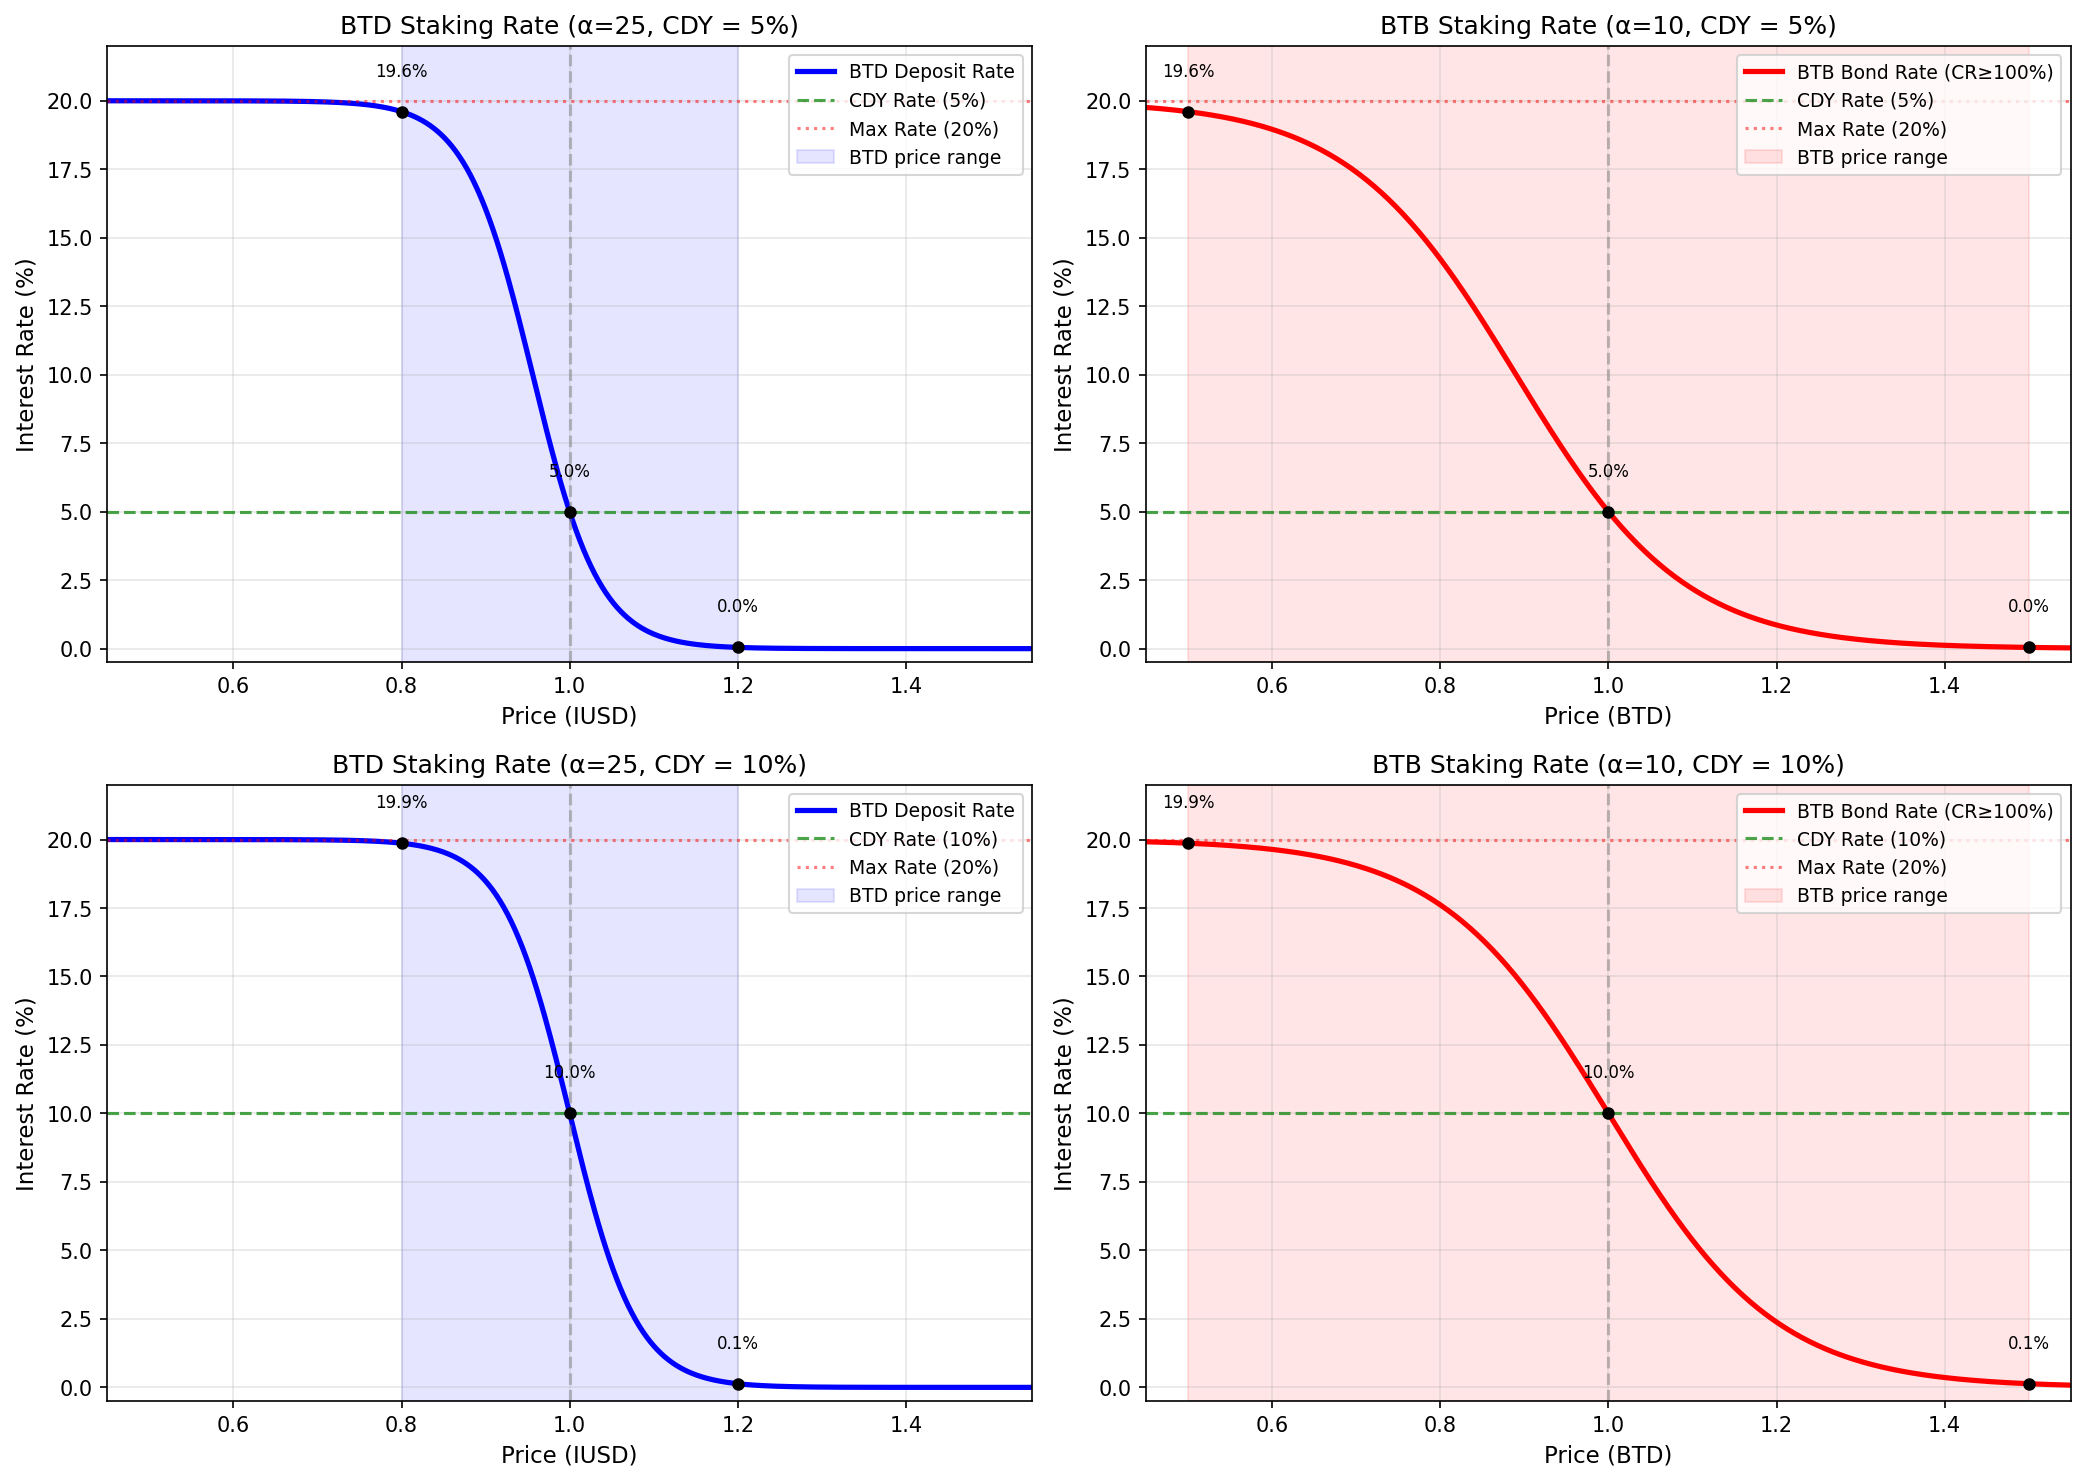
\includegraphics[width=\textwidth]{interest_rate_sigmoid.png}
  \caption{BTD and BTB staking interest rate curves at different collateral ratios. The shaded regions indicate the effective price ranges for each token.}
  \label{fig:interest-rate-curves}
\end{figure}

\paragraph{Rate Updates and Fees}
\begin{itemize}
  \item \textbf{Rate Updates:} Both rates are recalculated daily based on current CR and previous 24-hour TWAP prices obtained from on-chain oracles.
  \item \textbf{Interest Fee:} When depositors collect interest, an extra 5\% is minted as system fee and deposited into the treasury.
  \item Both interest pools' rewards mint new tokens, which enter vault total assets and are distributed to stakers through share price appreciation.
\end{itemize}

\subsubsection{Further Staking for Dual Yields}
After obtaining stBTD/stBTB, users can further stake them into the BRS mining pool (FarmingPool):
\begin{itemize}
  \item Stake stBTD → Continue enjoying BTD interest (through stBTD price appreciation) + Earn BRS mining rewards;
  \item Stake stBTB → Continue enjoying BTB interest (through stBTB price appreciation) + Earn BRS mining rewards;
  \item Dual yields require no additional operations, stToken share price grows automatically, BRS rewards can be claimed at any time.
\end{itemize}

This mechanism ensures users' funds only need to be transferred once to simultaneously receive interest earnings and mining rewards, greatly improving capital efficiency and user experience.

\subsection{Operation Delay and Security}
To prevent short-term interest rate attacks or reentrancy, there must be at least 5 blocks between reward withdrawals. Staking, withdrawal, and claiming operations are all protected by reentrancy guards and ownership controls, combined with pause, custody, and blacklist permissions in token contracts, enhancing compliance and security.

\section{Risk Hierarchy and Return Comparison}
\begin{center}
\begin{tabularx}{\textwidth}{l l l l}
\toprule
Token & Risk Level & Primary Backing Assets & Return Source \\
\midrule
BTD & Low & BTC, BTB, BRS & Deposit rate (based on CR) \\
BTB & Medium & BTD reserves & Bond rate (dynamically adjusted) \\
BRS & High & System residual equity & Mining output and treasury buyback \\
\bottomrule
\end{tabularx}
\end{center}
BTD enjoys the highest priority redemption order; BTB has priority redemption after collateral ratio recovery; BRS, as the residual claimant, bears the greatest risk but gains appreciation space through governance rights, fee buybacks, and ongoing mining incentives.

\section{Governance}

After the official genesis of the BRS system, there will be a beta testing period. During this period, to quickly fix bugs and add necessary features based on market demand, governance rights for the entire system will be controlled by the development team. Once the system develops to a certain stage and enters a stable period, the development team will transfer governance rights to the community. From then on, the system adopts an on-chain governance mechanism based on BRS tokens, ensuring the community can democratically participate in system parameter adjustments and protocol upgrade decisions. The governance architecture follows the OpenZeppelin Governor standard, providing transparent and auditable proposal and voting processes.

\subsection{Weak Governance Design Principles}

\textbf{The system adopts a ``weak governance'' style, hard-coding the vast majority of parameters at launch to make its behavior as close to Bitcoin's immutability as possible}. Governance capability is strictly limited to the minimum necessary scope:

\subsubsection{Parameter Solidification Strategy}
\begin{itemize}
  \item \textbf{Core Constants Fully Solidified} (immutable):
    \begin{itemize}
      \item All internal contract addresses (BTD, BTB, BRS, Treasury, Minter, Config, etc.)
      \item IUSD inflation parameters (2\% annual, monthly growth factor)
      \item BRS total supply cap (2.1 billion) and halving mechanism
      \item Core calculation algorithms and precision configurations
    \end{itemize}
  \item \textbf{System Constants} (static constant):
    \begin{itemize}
      \item Mathematical precision constants (18 decimal base)
      \item Time constants (seconds/days/years conversion)
      \item Safety ceilings (maximum deviation threshold 5\%, minimum deviation threshold 0.5\%)
    \end{itemize}
\end{itemize}

\subsubsection{Governable Parameters and Their Constraints}
A small number of parameters retain governance capability, but are strictly constrained by \textbf{security mechanisms}:

\textbf{1. External System Addresses} (with timelock):
\begin{itemize}
  \item Oracle addresses (Chainlink feeds, Pyth, Redstone) --- subject to 7-day timelock and whitelist
  \item DEX pool addresses (BTD/USDC, BTB/BTD, BRS/BTD, WBTC/USDC) --- subject to 7-day timelock
  \item These addresses are governable to allow upgrades when external systems change or migrate
\end{itemize}

\textbf{2. Price Deviation Tolerance} (default 1\%)
\begin{itemize}
  \item \textit{Boundary Check}: Can only be adjusted within 0.5\%--5\% range
  \item \textit{Unidirectional Tightening}: Can only lower the threshold, not raise it
  \item \textit{Cooldown Period}: At least 1 day between adjustments
  \item \textit{Event Log}: Complete record of each change
\end{itemize}

\textbf{3. BTD Minting Fee} (default 0.5\%)
\begin{itemize}
  \item \textit{Range Limit}: 0\%--10\%
  \item \textit{Cooldown Period}: At least 3 days between adjustments
\end{itemize}

\textbf{4. BTB Minimum Price Protection} (default 0.5 BTD)
\begin{itemize}
  \item \textit{Range Limit}: 0.3--0.7 BTD
  \item \textit{Cooldown Period}: At least 7 days between adjustments
\end{itemize}

\textbf{5. BTB Maximum Annual Rate} (default 20\%)
\begin{itemize}
  \item \textit{Range Limit}: 10\%--50\%
  \item \textit{Cooldown Period}: At least 7 days between adjustments
\end{itemize}

\textbf{6. Mining Allocation Weights}
\begin{itemize}
  \item \textit{Whitelist Restriction}: Can only adjust weights within predefined pool set
  \item \textit{Total Conservation}: Sum of all weights always equals 100\%
  \item \textit{Cooldown Period}: At least 14 days between adjustments
\end{itemize}

\textbf{7. Emergency Operations} (contract pause, blacklist)
\begin{itemize}
  \item \textit{Fast Track}: Can be quickly executed during security events, but requires multi-sig confirmation
  \item \textit{Timelock Exemption}: Pause operations are exempt from timelock, resume operations must go through complete governance process
  \item \textit{Transparency}: All operations are fully recorded in on-chain events
\end{itemize}

\subsubsection{Anti-Governance Abuse Mechanisms}
\begin{itemize}
  \item \textbf{Timelock Delay}: All governance proposals (except emergency pause) must go through at least 2 days of timelock delay before execution
  \item \textbf{Voting Power Snapshot}: Voting weight is determined at proposal creation, preventing flash loan attacks
  \item \textbf{Proposal Threshold}: Creating a proposal requires holding sufficient BRS (initially 250,000 BRS)
  \item \textbf{Quorum}: Proposal passage requires at least 4\% of total supply participating in voting
  \item \textbf{Proposal Cancellation Right}: When malicious proposals are discovered, creators or timelock administrators can cancel before execution
  \item \textbf{Whitelist Constraint}: All address-type parameters (such as backup oracles) can only switch within pre-approved whitelists
\end{itemize}

\subsubsection{Design Objectives}
Weak governance design pursues the following objectives:
\begin{itemize}
  \item \textbf{Predictability}: Users and developers can rely on the system's core behavior not being changed by governance
  \item \textbf{Immutability}: Key economic parameters (inflation rate, total supply cap) are as unmodifiable as Bitcoin
  \item \textbf{Minimal Trust}: Reduces trust assumptions about governors, lowers governance attack surface
  \item \textbf{Emergency Flexibility}: Retains minimum necessary capability to handle extreme market situations and security events
\end{itemize}

This design ensures the system is as stable and reliable as the Bitcoin protocol while retaining minimum flexibility to handle unknown risks.

\subsection{Governance Token Voting Rights}

BRS token integrates ERC20Votes extension, granting holders voting weight:
\begin{itemize}
  \item Voting weight equals the amount of BRS held (1 BRS = 1 vote);
  \item Voting power is implemented through delegation mechanism, holders can delegate voting power to themselves or other addresses;
  \item Voting power snapshot is determined at proposal creation, preventing token transfers during voting from affecting results;
  \item Supports offline signature voting (Permit feature), reducing participation costs.
\end{itemize}

\subsection{Governance Process}

The complete proposal lifecycle includes the following phases:

\subsubsection{Proposal Creation}
Any address holding sufficient BRS can create a proposal:
\begin{itemize}
  \item \textbf{Proposal Threshold:} Hold at least 250,000 BRS (adjustable by governance);
  \item \textbf{Proposal Content:} Includes target contract address, call data, and detailed description;
  \item \textbf{Proposal Types:} Supports parameter adjustment, protocol upgrade, fund allocation, and any other on-chain operations.
\end{itemize}

\subsubsection{Voting Delay Period}
After proposal creation, the system enters a 1-day voting delay period:
\begin{itemize}
  \item Determines voting power snapshot, preventing temporary token purchases to manipulate voting;
  \item Gives the community sufficient time to review proposal content;
  \item Automatically enters voting period after delay period ends.
\end{itemize}

\subsubsection{Voting Period}
Voting period lasts 7 days, addresses with voting power can vote:
\begin{itemize}
  \item \textbf{Voting Options:} For, Against, Abstain;
  \item \textbf{Voting Methods:} On-chain transaction or offline signature (EIP-712);
  \item \textbf{Vote Changes:} Can modify choice within voting period after voting.
\end{itemize}

\subsubsection{Quorum and Passing Conditions}
Proposal passage requires meeting both:
\begin{itemize}
  \item \textbf{Quorum:} At least 4\% of total supply participating in voting (based on supply at snapshot);
  \item \textbf{Majority For:} For votes $>$ Against votes (Abstain votes not counted).
\end{itemize}

\subsubsection{Timelock Queue}
Passed proposals are not executed immediately, but enter the timelock queue:
\begin{itemize}
  \item Proposal queues in timelock contract with minimum delay period (e.g., 2 days);
  \item During delay period, community can review upcoming operations and cancel through emergency proposal if issues are found;
  \item Timelock protects system from rapid attacks by malicious proposals.
\end{itemize}

\subsubsection{Proposal Execution}
After timelock delay period ends, anyone can trigger proposal execution:
\begin{itemize}
  \item Executor calls Governor contract's \texttt{execute()} function;
  \item Timelock contract verifies delay period has passed, executes on-chain operations specified in proposal;
  \item Execution results are recorded in on-chain events, fully transparent and auditable.
\end{itemize}

\subsection{Governance Scope}

System parameters and operations adjustable through on-chain governance include (but are not limited to):

\textbf{Economic Parameters:}
\begin{itemize}
  \item BTD minting fee ratio (default 0.5\%)
  \item BTB minimum price protection (default 0.5 BTD)
  \item BTB maximum annual rate cap (default 20\%)
  \item Interest fee ratio (default 5\%)
  \item Price deviation tolerance threshold (default 1\%)
\end{itemize}

\textbf{Mining Allocation:}
\begin{itemize}
  \item Allocation weights for each mining pool
  \item Fund allocation ratios (Treasury, Foundation, Team)
  \item Adding or removing mining pools
\end{itemize}

\textbf{Protocol Upgrades:}
\begin{itemize}
  \item Upgrade operations for UUPS upgradeable contracts (must go through timelock)
  \item Oracle contract address updates
  \item Addition of new feature modules
\end{itemize}

\textbf{Emergency Operations:}
\begin{itemize}
  \item Contract pause/resume (responding to security events)
  \item Blacklist management (compliance requirements)
  \item Treasury fund management (buyback, transfer, etc.)
\end{itemize}

\subsection{Governance Security Mechanisms}

To ensure governance security, the system employs multi-layer protection measures:

\begin{itemize}
  \item \textbf{Voting Power Snapshot:} Prevents flash loan attacks and temporary voting power purchases;
  \item \textbf{Timelock Delay:} Gives community sufficient time to discover and respond to malicious proposals;
  \item \textbf{Proposal Cancellation:} Proposal creators or timelock administrators can cancel proposals before execution;
  \item \textbf{Emergency Pause:} When serious security issues are discovered, contracts can be paused through fast governance process;
  \item \textbf{Upgradability:} Governor contract itself is upgradeable, supporting iterative optimization of governance mechanisms.
\end{itemize}

\subsection{Governance Parameters Overview}

\begin{center}
\begin{tabular}{ll}
\toprule
Parameter & Initial Value \\
\midrule
Proposal Threshold & 250,000 BRS \\
Voting Delay & 1 day \\
Voting Period & 7 days \\
Quorum & 4\% of total supply \\
Timelock Delay & 2 days (configurable) \\
Voting Method & Simple majority (For $>$ Against) \\
\bottomrule
\end{tabular}
\end{center}

All governance parameters can be adjusted through governance proposals themselves, enabling system self-evolution and optimization.

\section{Summary}
Chapters 3--6 of the whitepaper propose a three-layer defense architecture of ``BTC collateral + bond adjustment + governance token backstop''. The formulas, parameters, and sequence given in this document are fully aligned: BTD minting and redemption follow the pegging principle of $1\,\text{BTD}=1\,\text{IUSD}$; BTB regulates debt interest rates through price intervals; BRS is generated through a four-year halving mining mechanism while using treasury buybacks to absorb long-term risks.

\subsection{Core Advantages of Functional and Weak Governance}

The system design follows two core principles to ensure long-term stability and predictability:

\textbf{Functional Architecture} achieves clear separation of algorithms and state:
\begin{itemize}
  \item Core business logic (price calculation, collateral ratio calculation, IUSD adjustment, interest accumulation, etc.) encapsulated as pure function libraries
  \item Contract layer state minimized, storing only necessary addresses, balances, and accumulated values
  \item All calculation logic is deterministic, testable, and auditable
  \item Gas efficiency optimization: immutable parameter reading costs only 3 gas (vs 2100 gas for storage), saving 99.86\%
\end{itemize}

\textbf{Weak Governance Principle} anchors system behavior to Bitcoin-like immutability:
\begin{itemize}
  \item \textbf{46\% are static constants}: Mathematical precision, time conversion, safety ceilings, interest rate parameters, etc., determined at compile time
  \item \textbf{23\% of parameters fully solidified}: Core addresses, IUSD inflation rate, BRS total supply, etc., set as immutable at deployment, never changeable
  \item \textbf{31\% of parameters are governable}: A small number of parameters like external system addresses, fees, deviation thresholds, rate caps retain governance capability, but are strictly constrained by security mechanisms (boundary checks, cooldown periods, whitelist restrictions, event logs)
  \item \textbf{Unidirectional Tightening Principle}: Price deviation threshold can only be gradually tightened, not loosened, preventing governance from lowering security standards
  \item \textbf{Timelock Protection}: All governance operations (except emergency pause) must go through at least 2 days of timelock delay, giving the community sufficient reaction time
\end{itemize}

\subsection{Design Objectives Achieved}

Through the combination of functional and weak governance, the system achieves:
\begin{itemize}
  \item \textbf{Predictability}: Core economic parameters (2\% inflation rate, 2.1 billion BRS total supply) are as immutable as Bitcoin's 21 million cap
  \item \textbf{Transparency}: All algorithms presented in mathematical formula form, behavior is completely deterministic
  \item \textbf{Security}: Attack vectors like price manipulation and inflation rate tampering are completely eliminated
  \item \textbf{Minimal Trust}: Users need not trust that governors won't change core rules
  \item \textbf{Emergency Flexibility}: Retains minimum necessary capability to handle extreme situations (limited parameter adjustment, contract upgrades, emergency pause)
\end{itemize}

This design philosophy ensures the BRS system maintains the same level of stability and trustworthiness as the Bitcoin protocol while providing decentralized stablecoin services. Through on-chain governance mechanisms, the community can democratically adjust necessary parameters and drive protocol evolution within strict constraints. Therefore, as long as implementations follow the mechanisms and parameters specified in this document, they can remain consistent with the whitepaper and expand into various implementation schemes in the future.

\appendix

\section{Technical Appendix}

\subsection{Functional Architecture and Pure Function Library Layer}

The system adopts a functional programming paradigm, abstracting core business logic into pure function libraries, achieving separation of state and computation.

\subsubsection{Library Layer Design Principles}
\begin{itemize}
  \item \textbf{Pure Functionality}: All library functions do not read or write storage, only compute based on input parameters, ensuring determinism and testability
  \item \textbf{State Independence}: Library functions do not depend on contract state, can be independently tested and formally verified
  \item \textbf{Algorithm Transparency}: All calculation logic presented in mathematical formula form, behavior is completely predictable
  \item \textbf{Gas Optimization}: Library functions compile to inline code or delegatecall, avoiding state access overhead
\end{itemize}

\subsubsection{Core Function Libraries}

\textbf{PriceBlend (Price Aggregation Library):}
\begin{itemize}
  \item \texttt{median3(p1, p2, p3)}: Three-number median calculation
  \item \texttt{blendMultiSource(prices[], maxDeviation)}: Multi-source price median aggregation, supports 5+ oracle sources
  \item \texttt{validateSpotAgainstRef(spot, ref, maxBps)}: Spot price vs reference price deviation validation
  \item \texttt{validateAllWithinBounds(prices[], maxBps)}: Comprehensive deviation verification (O(n²) all price pair checks)
\end{itemize}

\textbf{IUSDMath (IUSD Calculation Library):}
\begin{itemize}
  \item \texttt{adjustmentFactor(currentPCE, basePCE, monthlyFactor, periods)}: Calculate adjustment factor based on PCE data
  \item \texttt{calculateIUSD(basePCE, currentPCE, targetRate, periods)}: Complete IUSD price calculation
  \item Boundary checks: PCE value $>$ 0, adjustment factor single-step change $\leq$ 5\%
\end{itemize}

\textbf{FeedValidation (Oracle Validation Library):}
\begin{itemize}
  \item \texttt{readAggregator(feed, maxStaleness)}: Chainlink feed reading and normalization
  \item \texttt{normalizeDecimals(value, fromDecimals, toDecimals)}: Precision conversion
  \item \texttt{checkFreshness(timestamp, maxAge)}: Data freshness verification
\end{itemize}

\textbf{OracleMath (Oracle Math Library):}
\begin{itemize}
  \item \texttt{normalizeAmount(amount, decimals, targetDecimals)}: General precision normalization
  \item \texttt{deviationWithin(value1, value2, maxBps)}: Deviation percentage calculation and determination
\end{itemize}

\textbf{CollateralMath (Collateral Ratio Calculation Library):}
\begin{itemize}
  \item \texttt{calculateCR(btcAmount, btcPrice, btdSupply, iusdPrice)}: Collateral ratio calculation
  \item \texttt{redeemAmounts(btdAmount, cr, btcPrice, btbPrice, brsPrice)}: Redemption asset portfolio calculation
\end{itemize}

\textbf{MintLogic / RedeemLogic (Minting/Redemption Logic Libraries):}
\begin{itemize}
  \item Encapsulate complete minting and redemption calculation logic
  \item Separate business logic from state management
  \item Facilitate unit testing and auditing
\end{itemize}

\textbf{InterestMath / RewardMath (Interest/Reward Calculation Libraries):}
\begin{itemize}
  \item \texttt{calculateInterest(principal, rate, timeDelta)}: Interest calculation
  \item \texttt{calculateReward(staked, totalStaked, rewardPerSecond, timeDelta)}: Mining reward calculation
  \item Precise accumulation algorithm based on block time
\end{itemize}

\textbf{PrecisionMath (Precision Handling Library):}
\begin{itemize}
  \item Safe multiplication and division at 18-digit precision
  \item Overflow protection and rounding error control
  \item Supports conversion between assets of different precisions
\end{itemize}

\subsubsection{Contract Layer Responsibilities}
The contract layer is only responsible for:
\begin{itemize}
  \item \textbf{Minimal State Management}: Store necessary addresses, balances, accumulated values, etc.
  \item \textbf{Permission Control}: Verify caller identity and operation permissions
  \item \textbf{Event Logging}: Record state changes and key operations
  \item \textbf{Library Function Calls}: Delegate computation to pure function libraries
\end{itemize}

\subsubsection{Layering Advantages}
\begin{itemize}
  \item \textbf{Testability}: Pure function libraries can be independently unit tested without contract deployment
  \item \textbf{Auditability}: Algorithm logic is clear, easy to manually review and formally verify
  \item \textbf{Upgradability}: During contract upgrades, library function logic remains unchanged, reducing risk
  \item \textbf{Gas Efficiency}: Inline functions avoid cross-contract calls, immutable parameters save 99.86\% reading cost
  \item \textbf{Composability}: Library functions can be reused across different contracts, maintaining consistency
\end{itemize}

\section{System Parameter List}

This appendix summarizes all core parameters in the BRS system, categorized by mutability into three types: static constants (constant), immutables (immutable), and governable variables (governable).

\subsection{Static Constants (Constant)}

Static constants are determined at compile time, written into contract bytecode, and permanently immutable. Primarily stored in the \texttt{Constants.sol} library.

\subsubsection{Precision Constants}

{\small
\begin{center}
\begin{longtable}{p{5.5cm}p{3cm}p{5.5cm}}
\toprule
Parameter Name & Value & Description \\
\midrule
\endhead
PRECISION\_18 & $10^{18}$ & 18-digit standard precision \\
PRECISION\_8 & $10^{8}$ & 8-digit precision (BTC) \\
PRECISION\_6 & $10^{6}$ & 6-digit precision (USDC/USDT) \\
SCALE\_WBTC\_TO\_NORM & $10^{10}$ & WBTC$\rightarrow$standard precision scale \\
SCALE\_USDC\_TO\_NORM & $10^{12}$ & USDC$\rightarrow$standard precision scale \\
BPS\_BASE & 10000 & Basis point base (100.00\%) \\
PERCENT\_BASE & 100 & Percentage base \\
\bottomrule
\end{longtable}
\end{center}
}

\subsubsection{Time Constants}

\begin{center}
\begin{longtable}{p{5cm}p{4cm}p{5cm}}
\toprule
Parameter Name & Value & Description \\
\midrule
\endhead
SECONDS\_PER\_YEAR & 31536000 & Seconds per year (365 days) \\
SECONDS\_PER\_DAY & 86400 & Seconds per day \\
SECONDS\_PER\_WEEK & 604800 & Seconds per week \\
ERA\_PERIOD & 126144000 & BRS halving cycle (4 years) \\
\bottomrule
\end{longtable}
\end{center}

\subsubsection{Inflation Parameter Constants}

{\small
\begin{center}
\begin{longtable}{p{6cm}p{5cm}p{3cm}}
\toprule
Parameter Name & Value & Description \\
\midrule
\endhead
ANNUAL\_INFLATION\_RATE & $2 \times 10^{16}$ & Annual inflation rate 2\% \\
MONTHLY\_GROWTH\_FACTOR & 1001651581301920174 & $1.02^{1/12}$ \\
\bottomrule
\end{longtable}
\end{center}
}

\subsubsection{Supply and Limit Constants}

{\small
\begin{center}
\begin{longtable}{p{6.5cm}p{3cm}p{4.5cm}}
\toprule
Parameter Name & Value & Description \\
\midrule
\endhead
BRS\_MAX\_SUPPLY & $2.1 \times 10^{27}$ & BRS maximum supply (2.1 billion) \\
MIN\_BTC\_AMOUNT & 1 & Minimum BTC operation amount \\
MIN\_ETH\_AMOUNT & $10^{10}$ & Minimum ETH operation amount \\
MIN\_USD\_VALUE & $10^{15}$ & Minimum USD value \\
MIN\_STABLECOIN\_18\_AMOUNT & $10^{15}$ & 18-digit stablecoin minimum amount \\
MIN\_STABLECOIN\_6\_AMOUNT & 1000 & 6-digit stablecoin minimum amount \\
MAX\_WBTC\_AMOUNT & $10^{12}$ & WBTC single transaction maximum \\
MAX\_ETH\_AMOUNT & $10^{23}$ & ETH single transaction maximum \\
MAX\_STABLECOIN\_18\_AMOUNT & $10^{27}$ & 18-digit stablecoin maximum amount \\
MAX\_STABLECOIN\_6\_AMOUNT & $10^{15}$ & 6-digit stablecoin maximum amount \\
MAX\_USD\_VALUE & $10^{27}$ & Single transaction maximum USD value \\
\bottomrule
\end{longtable}
\end{center}
}

\subsubsection{Oracle Security Constants}

{\small
\begin{center}
\begin{longtable}{p{6.5cm}p{3cm}p{4.5cm}}
\toprule
Parameter Name & Value & Description \\
\midrule
\endhead
MAX\_DEVIATION\_CEILING & 500 bps & Price deviation ceiling (5\%) \\
MIN\_DEVIATION\_FLOOR & 50 bps & Price deviation floor (0.5\%) \\
DEVIATION\_UPDATE\_COOLDOWN & 1 day & Deviation adjustment cooldown \\
PYTH\_MAX\_STALENESS & 60 seconds & Pyth price maximum staleness \\
PYTH\_MAX\_CONF\_RATIO & 100 & Pyth confidence threshold (1\%) \\
TWAP\_PERIOD & 30 minutes & TWAP observation period \\
\bottomrule
\end{longtable}
\end{center}
}

\subsubsection{Interest Rate Constants (InterestPool)}

{\small
\begin{center}
\begin{longtable}{p{6cm}p{3.5cm}p{4.5cm}}
\toprule
Parameter Name & Value & Description \\
\midrule
\endhead
\multicolumn{3}{l}{\textit{BTB CR-Based Parameters}} \\
BTB\_CR\_THRESHOLD & $10^{18}$ & CR threshold (100\%) \\
BTB\_CR\_MIN & $2 \times 10^{17}$ & Minimum CR (20\%) \\
BTB\_CR\_DIVISOR & $8 \times 10^{17}$ & CR divisor for linear factor (0.8) \\
\midrule
\multicolumn{3}{l}{\textit{Rate Update Parameters}} \\
RATE\_UPDATE\_INTERVAL & 86400 & Rate recalculation interval (24h) \\
TWAP\_WINDOW\_DEFAULT & 86400 & TWAP observation window (24h) \\
\bottomrule
\end{longtable}
\end{center}
}

\subsubsection{Governance Constants}

\begin{center}
\begin{longtable}{p{5cm}p{4cm}p{5cm}}
\toprule
Parameter Name & Value & Description \\
\midrule
\endhead
Voting Delay & 1 day & Proposal creation to voting start \\
Voting Period & 1 week & Voting duration \\
Proposal Threshold & 250,000 BRS & Tokens required to create proposal \\
Quorum & 4\% & Required voting participation ratio \\
Timelock Delay & 2 days & Proposal passage to execution \\
SHARE\_BASE & 100 & Fund allocation base \\
\bottomrule
\end{longtable}
\end{center}

\subsubsection{IUSD Manual Override Security Constants}

\begin{center}
\begin{longtable}{p{5.5cm}p{3.5cm}p{5cm}}
\toprule
Parameter Name & Value & Description \\
\midrule
\endhead
MIN\_OVERRIDE\_INTERVAL & 7 days & Manual override minimum interval \\
MAX\_MANUAL\_DEVIATION & 5\% & Manual adjustment maximum deviation \\
\bottomrule
\end{longtable}
\end{center}

\subsection{Immutables (Immutable)}

Immutables are set through the constructor at contract deployment and never changeable afterward. Storage cost is only 3 gas (vs 2100 gas for storage).

\subsubsection{Core Token Addresses (ConfigCore)}

\begin{center}
\begin{longtable}{p{4cm}p{10cm}}
\toprule
Parameter Name & Description \\
\midrule
\endhead
wbtcAddr & Wrapped BTC token address \\
btdAddr & Stablecoin BTD token address \\
btbAddr & Bond token BTB token address \\
brsAddr & Governance token BRS token address \\
wethAddr & Wrapped ETH token address \\
usdcAddr & USDC stablecoin address \\
usdtAddr & USDT stablecoin address \\
\bottomrule
\end{longtable}
\end{center}

\subsubsection{Core Contract Addresses (ConfigCore)}

\begin{center}
\begin{longtable}{p{5cm}p{9cm}}
\toprule
Parameter Name & Description \\
\midrule
\endhead
treasuryAddr & Treasury contract address \\
minterAddr & Minting and redemption contract address \\
priceOracleAddr & Price oracle contract address \\
idealUsdManagerAddr & IUSD manager address \\
interestPoolAddr & Interest pool contract address \\
stakingRouterAddr & Staking router contract address \\
farmingPoolAddr & Mining pool contract address \\
stBtdAddr & stBTD vault address \\
stBtbAddr & stBTB vault address \\
governorAddr & Governance contract address \\
twapOracleAddr & TWAP oracle address \\
\midrule
\multicolumn{2}{l}{\textit{DEX Pool Addresses}} \\
poolBtdUsdc & BTD-USDC trading pair (for BTD price) \\
poolBtbBtd & BTB-BTD trading pair (for BTB price) \\
poolBrsBtd & BRS-BTD trading pair (for BRS price) \\
\bottomrule
\end{longtable}
\end{center}

\subsubsection{Mining Parameters (FarmingPool)}

\begin{center}
\begin{longtable}{p{4cm}p{10cm}}
\toprule
Parameter Name & Description \\
\midrule
\endhead
startTime & Mining start timestamp \\
\bottomrule
\end{longtable}
\end{center}

\subsection{Governable Variables (Governable)}

Governable variables can be adjusted at runtime through governance mechanisms, but are strictly constrained: boundary checks, cooldown periods, whitelist restrictions, and event logs.

\subsubsection{Fee Parameters (ConfigGov)}

\begin{center}
\begin{longtable}{p{4cm}p{2.5cm}p{2.5cm}p{5cm}}
\toprule
Parameter Name & Default & Range & Description \\
\midrule
\endhead
mintFeeBp & 50 bps & 0--1000 bps & Minting fee (0.5\%) \\
redeemFeeBp & 50 bps & 0--1000 bps & Redemption fee (0.5\%) \\
interestFeeBp & 500 bps & 0--2000 bps & Interest fee (5\%) \\
\bottomrule
\end{longtable}
\end{center}

\subsubsection{Price Protection Parameters (ConfigGov)}

{\small
\begin{center}
\begin{longtable}{p{5cm}p{2.5cm}p{3cm}p{3.5cm}}
\toprule
Parameter Name & Default & Range & Description \\
\midrule
\endhead
minBtbPrice & 0.5 BTD & 0.3--0.7 BTD & BTB minimum price protection \\
pceMaxDeviation & 2\% & 0--10\% & PCE maximum deviation rate \\
\bottomrule
\end{longtable}
\end{center}
}

\subsubsection{External Oracle Address Parameters (ConfigGov)}

External oracle addresses are governable to allow upgrades when external systems change. All changes are subject to 7-day timelock and whitelist restrictions.

\begin{center}
\begin{longtable}{p{5cm}p{9cm}}
\toprule
Parameter Name & Description \\
\midrule
\endhead
pceFeedAddr & Chainlink PCE oracle address \\
chainlinkBtcUsdAddr & Chainlink BTC/USD price feed \\
chainlinkWbtcBtcAddr & Chainlink WBTC/BTC price feed \\
pythWbtcAddr & Pyth WBTC price feed address \\
redstoneWbtcAddr & Redstone WBTC price feed address \\
\bottomrule
\end{longtable}
\end{center}

\subsubsection{DEX Pool Address Parameters (ConfigGov)}

DEX pool addresses are governable to allow upgrades when liquidity migrates. All changes are subject to 7-day timelock.

\begin{center}
\begin{longtable}{p{4.5cm}p{9.5cm}}
\toprule
Parameter Name & Description \\
\midrule
\endhead
poolWbtcUsdcAddr & WBTC-USDC trading pair (for WBTC price) \\
\bottomrule
\end{longtable}
\end{center}

\subsubsection{Oracle Runtime Parameters (PriceOracle)}

\begin{center}
\begin{longtable}{p{4.5cm}p{2.5cm}p{3cm}p{4cm}}
\toprule
Parameter Name & Default & Constraint & Description \\
\midrule
\endhead
maxDeviationBps & 100 bps & Can only tighten & Price deviation tolerance \\
useTwap & true & Boolean & TWAP mode switch \\
\bottomrule
\end{longtable}
\end{center}

\subsubsection{Interest Rate Parameters (InterestPool)}

\begin{center}
\begin{longtable}{p{4.5cm}p{3cm}p{6.5cm}}
\toprule
Parameter Name & Default & Description \\
\midrule
\endhead
btdMaxRateBps & 2000 bps & BTD maximum rate (20\%), adjustable 1000--3000 bps \\
btbMaxRateBps & 2000 bps & BTB maximum rate (20\%), adjustable 1000--3000 bps \\
twapWindow & 24 hours & TWAP observation window (adjustable 12--48 hours) \\
\bottomrule
\end{longtable}
\end{center}

\textbf{Note:} BTD and BTB rates are calculated algorithmically using Sigmoid functions based on 24-hour TWAP prices and collateral ratio (CR). Base rate is $r_{default} \times (1 + \Delta_{CR})$ where $r_{default} = 5\%$. BTD range is 2\%--10\% with $\Delta_{CR} = (1-CR)/0.8$. BTB range is 2\%--20\% with 3x $\Delta_{CR}$ multiplier for higher risk compensation. Both reach 2\% minimum when CR $\geq$ 150\%.

\subsubsection{Mining Allocation Parameters (FarmingPool)}

\begin{center}
\begin{longtable}{p{4cm}p{10cm}}
\toprule
Parameter Name & Description \\
\midrule
\endhead
fundAddrs[] & Fund address array (Treasury, Foundation, Team) \\
fundShares[] & Fund allocation ratios (base 100, sum $\leq$100) \\
poolInfo[].allocPoint & Allocation weight for each pool \\
totalAllocPoint & Total allocation weight \\
\bottomrule
\end{longtable}
\end{center}

\subsubsection{Governance Runtime Parameters}

\begin{center}
\begin{longtable}{p{4.5cm}p{9.5cm}}
\toprule
Parameter Name & Description \\
\midrule
\endhead
Voting Delay & Adjustable via governance proposal \\
Voting Period & Adjustable via governance proposal \\
Proposal Threshold & Adjustable via governance proposal \\
Quorum Ratio & Adjustable via governance proposal \\
\bottomrule
\end{longtable}
\end{center}

\subsubsection{IUSD Parameters (IdealUSDManager)}

\begin{center}
\begin{longtable}{p{5cm}p{9cm}}
\toprule
Parameter Name & Description \\
\midrule
\endhead
iusdValue & Current IUSD value (updatable via updateIUSD) \\
authorizedUpdaters[] & Authorized updaters whitelist \\
updaterWhitelistEnabled & Whitelist enable switch \\
\bottomrule
\end{longtable}
\end{center}

\subsubsection{Treasury Parameters (Treasury)}

\begin{center}
\begin{longtable}{p{4cm}p{10cm}}
\toprule
Parameter Name & Description \\
\midrule
\endhead
routerAddr & Uniswap V2 Router address (for buybacks) \\
\bottomrule
\end{longtable}
\end{center}

\subsection{Parameter Classification Statistics}

\begin{center}
\begin{tabular}{lcc}
\toprule
Category & Count & Percentage \\
\midrule
Static Constants (constant) & $\sim$43 & $\sim$46\% \\
Immutables (immutable) & $\sim$22 & $\sim$23\% \\
Governable Variables (governable) & $\sim$29 & $\sim$31\% \\
\midrule
\textbf{Total} & \textbf{$\sim$94} & \textbf{100\%} \\
\bottomrule
\end{tabular}
\end{center}

\textbf{Design Notes:}

Approximately 69\% of system parameters are solidified at deployment (constant + immutable), with only 31\% retaining governance capability. This ``weak governance'' design ensures:

\begin{itemize}
  \item \textbf{Predictability}: Users and developers can rely on the system's core behavior not being changed by governance
  \item \textbf{Immutability}: Key economic parameters are as unmodifiable as Bitcoin
  \item \textbf{Minimal Trust}: Reduces trust assumptions about governors, lowers attack surface
  \item \textbf{Gas Optimization}: Immutable parameter reading costs only 3 gas, saving 99.86\%
  \item \textbf{Emergency Flexibility}: Retains minimum necessary adjustment capability for extreme situations
\end{itemize}

\end{document}
